\appendix
\section{Derivations}
\label{app:proofs}

\subsection{The LRU hit condition}

Order the keys by their most recent access. This is the LRU stack. A request to key
$k$ hits exactly when $k$ is in the first $C$ positions, because those are the $C$
distinct objects the cache holds. The number of distinct keys accessed after $k$'s
previous access and before the current one is exactly the number of keys that have
been touched since $k$, so $k$ is at depth $R_i$ in the stack. It is among the first
$C$ positions if and only if $R_i<C$. A key never accessed before is not in the
stack and misses at every finite $C$. Summing the indicator over requests gives
$\mathrm{MRC}(C)=\Pr(R\ge C)$.

\subsection{The grouped likelihood}
\label{app:grouped}

For one request with distance in bin $b$ and hazard $h_j$ in bin $j$, the per-step
likelihood is
\[
  \Bigl(\prod_{j<b}(1-h_j)\Bigr)\,h_b .
\]
Taking logs gives $\sum_{j<b}\log(1-h_j)+\log h_b$, a sum of one term per bin at
risk. The grouped form fits a binary classifier on those terms, with label 1 at $b$
and 0 before it. It is exact when $h$ is constant inside a bin; otherwise the
within-bin variation is the approximation error, and it shrinks as bins narrow. The
per-step expansion is the same construction at unit resolution and is used only as a
support check, because its row count grows with distance rather than with bin count.

\subsection{Why the forward event is biased here}
\label{app:forward}

The forward event asks whether the key is accessed again before the window ends.
That event is a different random variable from the backward distance: the two have
the same distribution only under stationarity, and the window truncates them
differently. A request early in the window whose key never recurs is censored at a
large bound, while the same request's backward distance may be small. Fitting the
forward hazard therefore estimates the distribution of a quantity the curve is not a
survival function of. The measured gap is in \cref{app:limitations}.

\subsection{Corrections and limitations}
\label{app:limitations}

\textbf{The forward-event target is biased.} The first implementation modelled
whether a key would be requested again before the window ended. That is a different
distribution from the backward distance the curve is a survival function of. It
produced test MAE 0.170 with a systematic optimistic bias of +0.170 on cluster45;
targeting the backward distance produced 0.005. The comparison is reported because
the error is not visible from the fitted model alone.

\textbf{A capacity grid inside a bin is a measurement error, not a model error.} The
first grid was log-spaced independently of the bins. Re-evaluating the same fitted
booster on bin upper edges cut cluster26's worst error from 0.147 to 0.021 and
cluster45's from 0.005 to 0.0003. The grid is now aligned.

\textbf{Four traces, one window each.} Every number is a within-trace fit on a
five-million-request window. Distances above the window are unobservable, which is
why every caption states the window and why the grid stops below $b_{M-1}$. The
cluster52 shard is 13.4 billion requests (93 GB compressed); only its first five
million are analysed, so nothing here is a claim about that cluster's full week or
about the reuse distances beyond the window.

\textbf{Cold-heavy workloads have a ceiling.} The hit ratio cannot exceed $1-p_c$.
On cluster10 that ceiling is 50\%, so a 90\% target is not a modelling problem. This
is why provisioning targets are stated relative to the ceiling.

\textbf{Tuning is bounded.} Optuna ran 15 trials on a four-million-row subsample of
cluster45, not 60 at full budget. The default parameters already reached the accuracy
gate, so the study is evidence that the search works, not the source of the headline
model. The best trial reached validation MAE 0.00036 against 0.00042 for the shipped
defaults, a 13\% improvement that is available but not used, so that every row of
\cref{tab:methods} shares one protocol.

\textbf{The single-row row of \cref{tab:methods} is an oracle.} It is included to
bound the risk-set expansion, and it is excluded from every headline comparison.

\textbf{Calibration was pre-registered and is not reported.} The statistical skeleton
pre-registered per-request calibration, Brier score and its integral over the bins, as
a secondary acceptance metric; neither is reported in this document, every reported
metric is curve-level (MAE, MAX, bias, MRE, ABC) or the provisioning decision, and the
calibration figure code was removed as unused.

\subsection{Reproduction}
\label{app:repro}

\begin{verbatim}
make check
mrc train cluster45 --rounds 300 --rows 20000000
mrc train cluster26 --rounds 300 --rows 20000000
mrc train cluster10 --rounds 300 --rows 20000000
mrc tune cluster45 --trials 15 --rounds 150 --rows 4000000
mrc interpret cluster45 --requests 600000 --rounds 150
mrc plots
cd report && latexmk -pdf main.tex
\end{verbatim}

% generated by scripts/full_metrics_table.py; do not edit
\begin{table}[t]
\centering
\scriptsize
\caption{Every metric on every trace and estimator, test block, on the frozen capacity grid of each trace. ABC is the log-normalised area between curves.}
\label{tab:full-metrics}
\begin{tabular}{@{}l l r r r r r@{}}
\toprule
Trace & Estimator & MAE & MAX & bias & MRE & ABC \\
\midrule
cluster45 & hazard & 0.00027 & 0.00107 & -0.00017 & 0.0005 & 0.0003 \\
cluster45 & Kaplan-Meier & 0.02000 & 0.03429 & -0.01645 & 0.0356 & 0.0202 \\
cluster45 & hit-count & 0.10968 & 0.19838 & -0.07341 & 0.1838 & 0.1139 \\
\midrule
cluster26 & hazard & 0.00548 & 0.02057 & -0.00539 & 0.0106 & 0.0053 \\
cluster26 & Kaplan-Meier & 0.01178 & 0.01537 & -0.01178 & 0.0201 & 0.0119 \\
cluster26 & hit-count & 0.07927 & 0.27053 & +0.04805 & 0.1477 & 0.0799 \\
\midrule
cluster52 & hazard & 0.00027 & 0.00079 & +0.00020 & 0.0007 & 0.0003 \\
cluster52 & Kaplan-Meier & 0.02481 & 0.04035 & -0.02481 & 0.0614 & 0.0247 \\
cluster52 & hit-count & 0.11342 & 0.25439 & -0.00889 & 0.2352 & 0.1132 \\
\midrule
cluster10 & hazard & 0.00772 & 0.01902 & -0.00772 & 0.0127 & 0.0092 \\
cluster10 & Kaplan-Meier & 0.04387 & 0.12042 & -0.04387 & 0.0623 & 0.0713 \\
cluster10 & hit-count & 0.07930 & 0.33206 & -0.06852 & 0.1112 & 0.1418 \\
\bottomrule
\end{tabular}
\end{table}


\Cref{tab:full-metrics} lists every metric on every trace, including the bias and
the log-normalised area between curves that the main text omits.

% generated by scripts/noise_floor.py; do not edit
\begin{table}[t]
\centering
\footnotesize
\caption{Model error against the sampling noise of the truth curve. $n$ is the number of eligible requests in the test block and $\mathrm{SE}$ the median binomial standard error of the empirical survival curve over its capacities, $\sqrt{p(1-p)/n}$, a lower bound on the true error of the truth because requests are serially dependent. A ratio below one means the model is inside the resolution of the block.}
\label{tab:noise}
\begin{tabular}{@{}l r r l r r@{}}
\toprule
Trace & $n$ & $\mathrm{SE}$ & Estimator & MAE/$\mathrm{SE}$ & within $1\,\mathrm{SE}$ \\
\midrule
cluster45 & \num{444781} & \num{7.35e-04} & Hazard GBDT & 0.36 & 23/24 \\
 & & & Kaplan-Meier & 27.22 & 0/24 \\
 & & & Hit-count & 149.28 & 0/24 \\
\midrule
cluster26 & \num{692522} & \num{5.53e-04} & Hazard GBDT & 9.91 & 1/24 \\
 & & & Kaplan-Meier & 21.31 & 0/24 \\
 & & & Hit-count & 143.33 & 0/24 \\
\midrule
cluster52 & \num{637941} & \num{5.44e-04} & Hazard GBDT & 0.50 & 21/24 \\
 & & & Kaplan-Meier & 45.59 & 0/24 \\
 & & & Hit-count & 208.37 & 0/24 \\
\midrule
cluster10 & \num{375008} & \num{8.14e-04} & Hazard GBDT & 9.48 & 3/12 \\
 & & & Kaplan-Meier & 53.88 & 1/12 \\
 & & & Hit-count & 97.40 & 0/12 \\
\bottomrule
\end{tabular}
\end{table}


\begin{center}
\begin{minipage}{\linewidth}
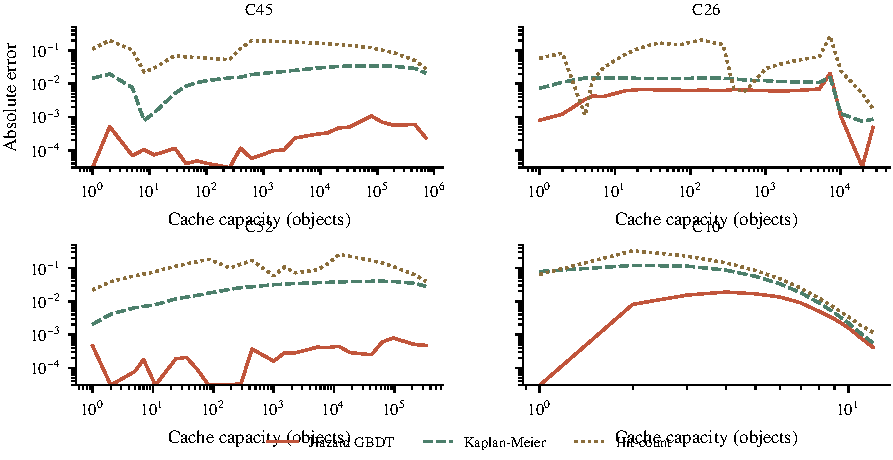
\includegraphics[width=\linewidth]{figures/cluster-error.pdf}
\captionof{figure}{Absolute curve error against capacity, log-log, one panel per
trace. Hazard GBDT solid, Kaplan-Meier dashed, hit-count dotted. Exact zeros are
floored at $3\times10^{-5}$, below every measured hazard error.}
\label{fig:cluster-error}
\end{minipage}
\end{center}

\subsection{Capacity ratio figure}
\label{app:capacity-figure}

\begin{center}
\begin{minipage}{0.62\linewidth}
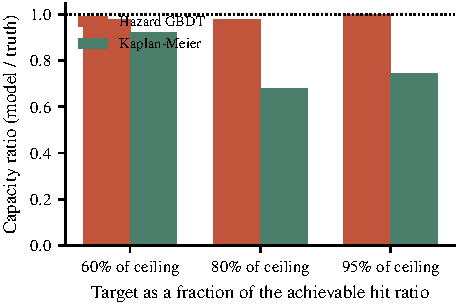
\includegraphics[width=\linewidth]{figures/capacity-ratio.pdf}
\captionof{figure}{Capacity ratio at three targets, median over the four traces,
with parity dotted. Below one is under-provisioning.}
\label{fig:capacity-ratio}
\end{minipage}
\end{center}

\subsection{Trace design numbers}
\label{app:traces}

\begin{table}[h]
\centering
\footnotesize
\sisetup{group-separator={,},group-minimum-digits=4}
\caption{The four traces, first 5{,}000{,}000 requests each. Eligible is the
fraction with a previous access inside the window; $p_c$ is its complement and is
the compulsory mass. $R$ is the backward reuse distance in objects. Bins and grid
points are realised counts; $b_{M-1}$ is the lower edge of the overflow bin, and
every reported capacity is below it.}
\label{tab:traces}
\begin{tabular}{@{}l r r r r r r r r@{}}
\toprule
Trace & {Keys} & {Mean object (B)} & {Eligible} & {$p_c$} & {$R$ p50} & {$R$ p99} & {Bins / grid} \\
\midrule
cluster45 & \num{2158200} & \num{91} & 0.568 & 0.432 & \num{4} & \num{1008186} & 33 / 24 \\
cluster26 & \num{394747} & \num{1046} & 0.921 & 0.079 & \num{472} & \num{17709} & 33 / 24 \\
cluster52 & \num{932119} & \num{252} & 0.814 & 0.186 & \num{1097} & \num{488644} & 33 / 24 \\
cluster10 & \num{2500051} & \num{1289} & 0.500 & 0.500 & \num{1} & \num{8} & 14 / 12 \\
\bottomrule
\end{tabular}
\end{table}
